\chapter{Model}
To make the quadcopter have a steady flight it is convenient to derive a model of the system, so the physical behavior of the quadcopter is described. From this, a control system must be designed such that the desired flying characteristics are obtained. The model is derived in this chapter.

First, an overview is presented. Then, the model is derived and lastly, it is linearized as this is necessary to be able to design a linear control system. The model and the linearized model are compared in simulations. This ensures that the linear approximation yields acceptable results.

\section{Model overview}
The model is split into two sub models. One being an angular model and the other is a translational velocity model. These models are later combined to fully simulate the response of the system.
\begin{figure}[H]
\centering
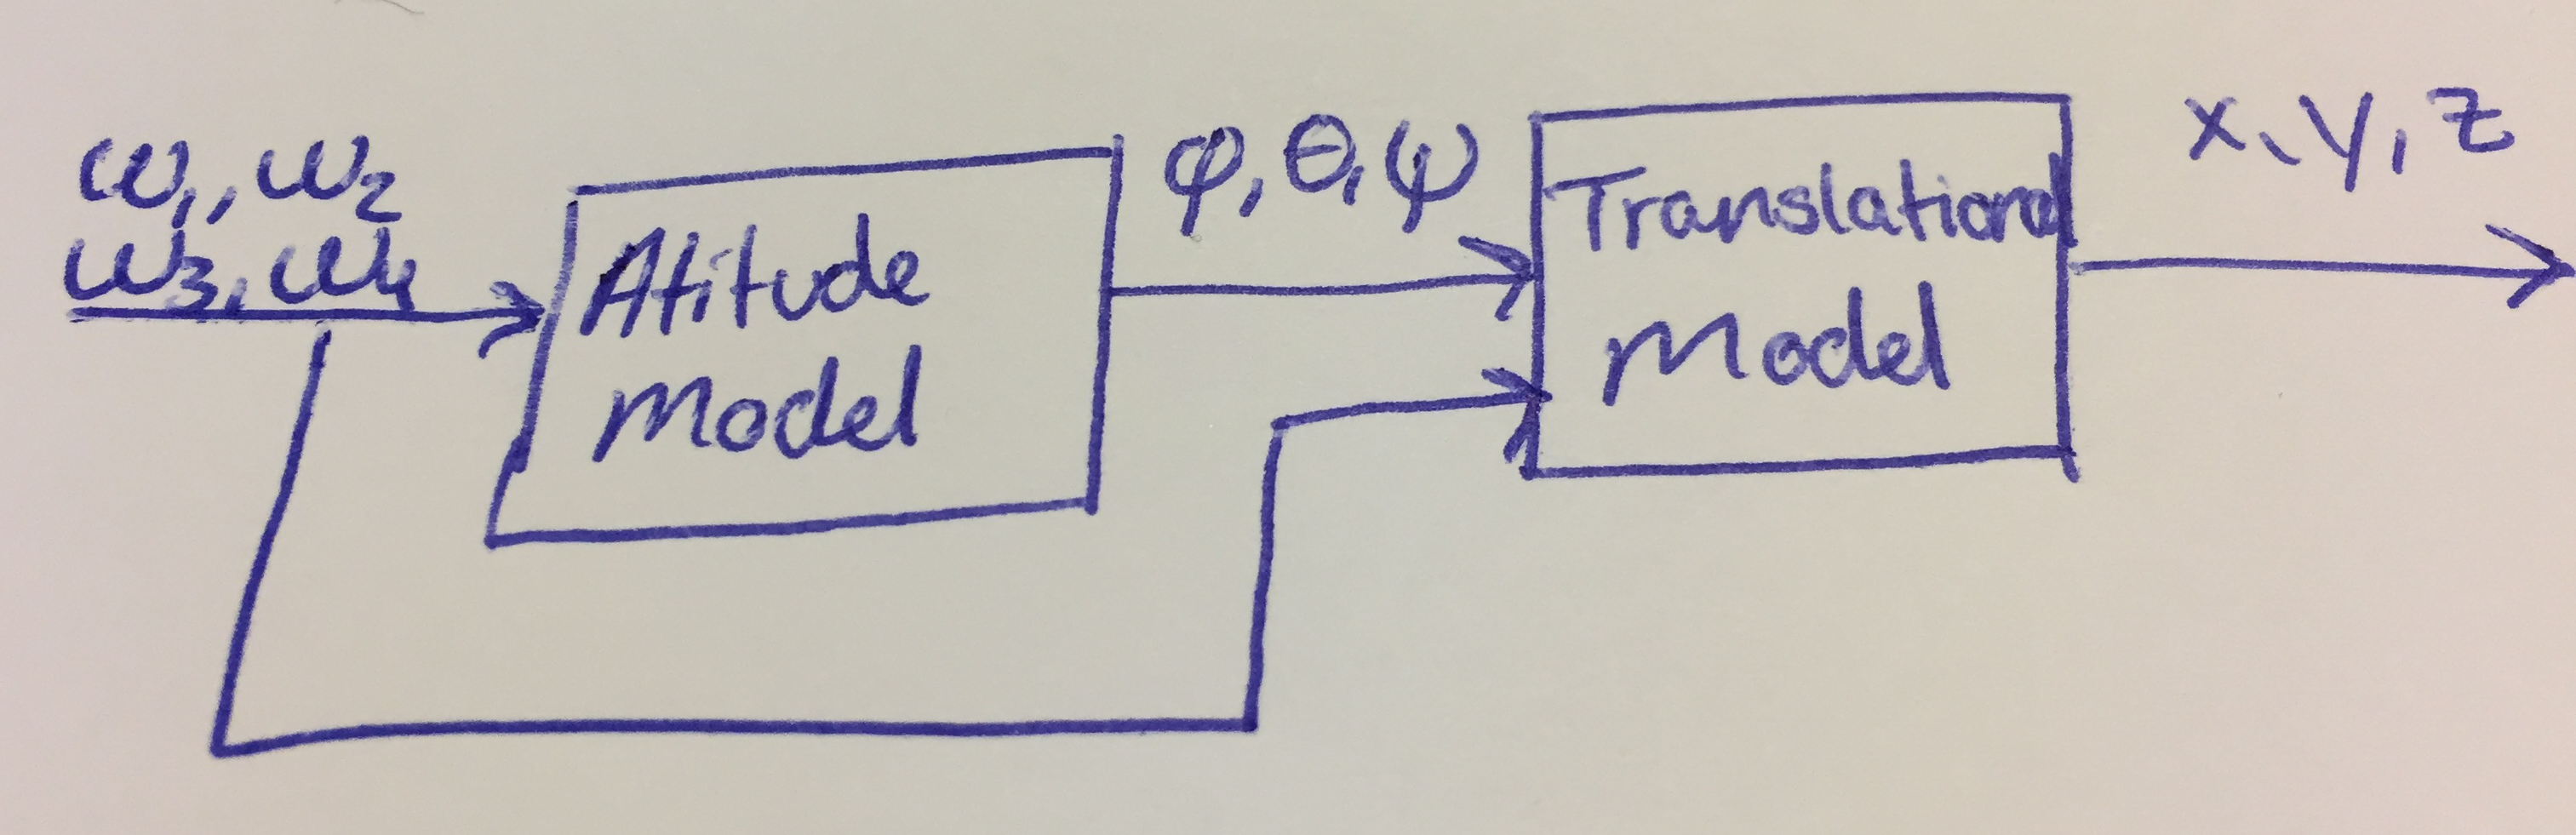
\includegraphics[scale=0.1]{figures/modeloverview.PNG}
\caption{Overview of how the model is split.}
\label{sss}
\end{figure}
Another consideration to be made before modeling the quadcopter is the usage of two coordinate frames. A body frame, that is fixed to the flying object and an inertial frame, that is fixed to the Vicon room. 

Using these two frames is necessary, as it is desired to know where the quadcopter is within the inertial frame to determine its position. To obtain the orientation of the quadcopter, the body frame's orientation compared to the inertial frame yields the angles of roll, pitch and yaw. 
%Angle and Linear
%Explain the two frames and include drawing showing them
%Flow of the chapter

%\Figref{diagramQuad} shows a representation of the quadcopter where two reference systems, inertial and body, can be seen, as well as the conventions for angles of rotation and forces. \Figref{diagramTorque} shows the body from above and includes the chosen convention for the torques produced by the propellers.
%
%\begin{minipage}{\linewidth}
%	\begin{minipage}{0.45\linewidth}
%		\begin{figure}[H]
%			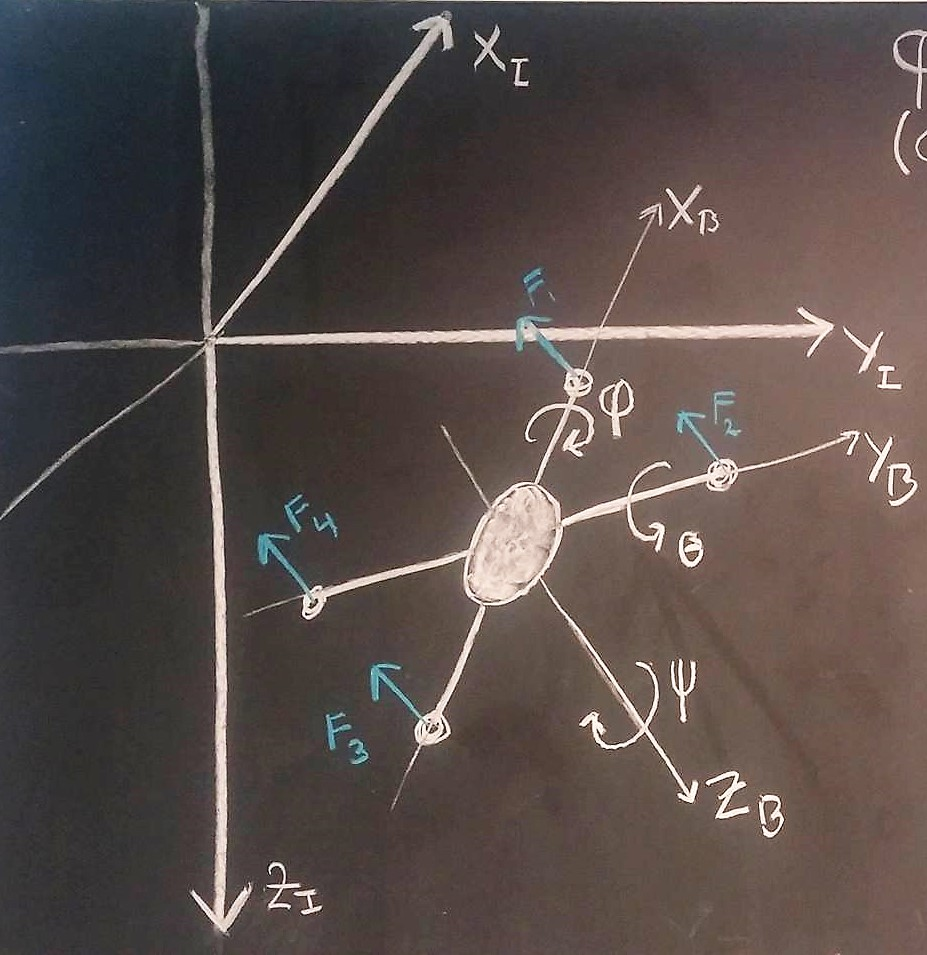
\includegraphics[scale=.27]{figures/drone_diagram}
%			\centering
%			\captionsetup{justification=centering}
%			\captionof{figure}{Diagram of the quadcopter which includes inertial and body reference systems, as well as the references for the angles (roll, pitch and yaw) and the thrust forces produced by the propeller. }
%			\label{diagramQuad}
%		\end{figure}
%	\end{minipage}
%	\hspace{0.03\linewidth}
%	\begin{minipage}{0.45\linewidth}
%		\begin{figure}[H] \vspace{16mm}
%			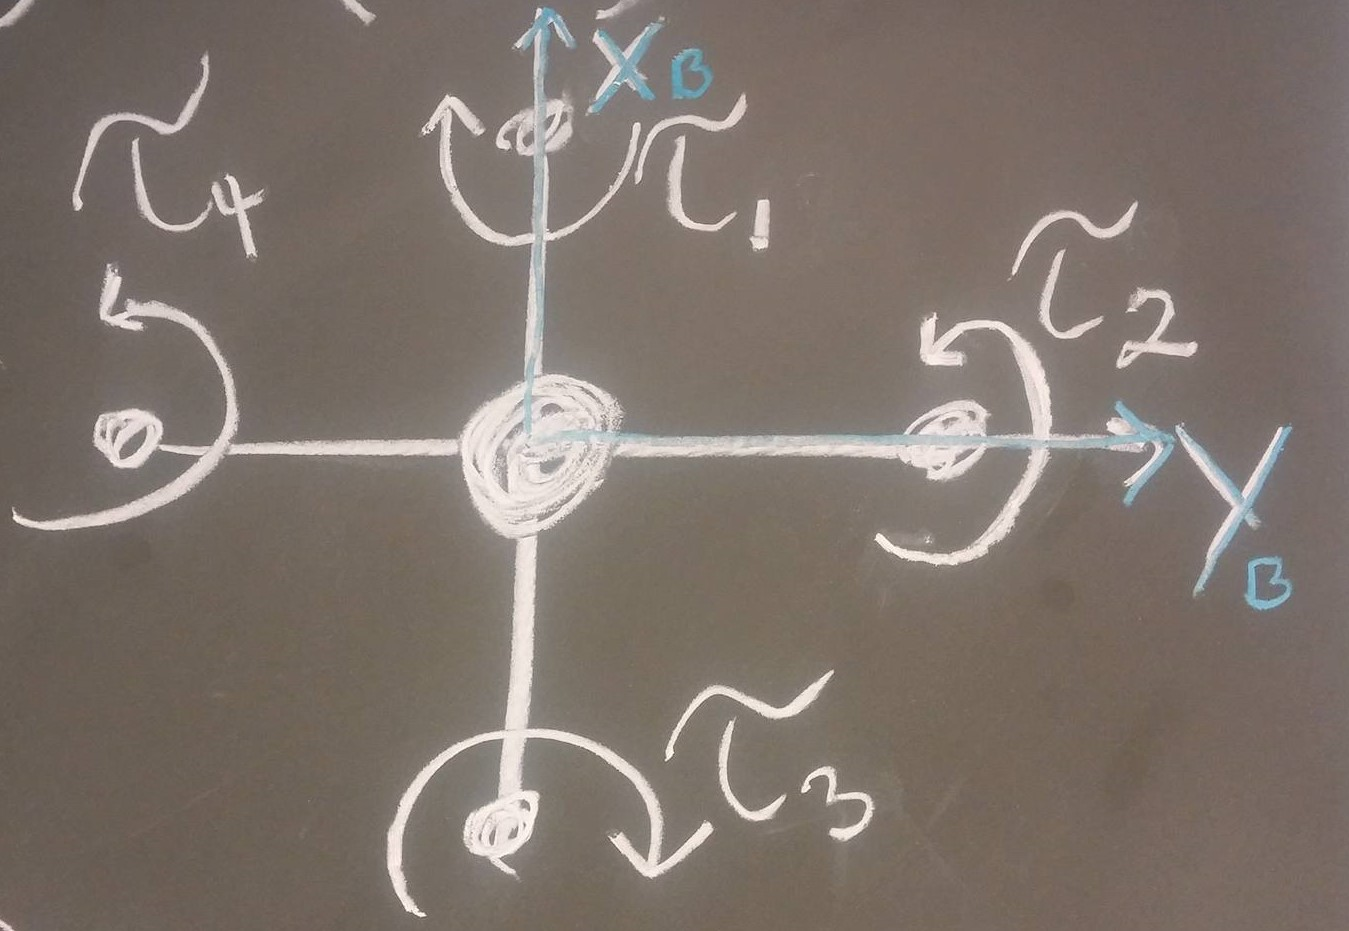
\includegraphics[scale=.18]{figures/torques_diagram}
%			\centering
%			\captionsetup{justification=centering}
%			\captionof{figure}{Diagram of the quadcopter from above, with the references for the torques produced by the drag force at the propeller.}
%			\label{diagramTorque}
%		\end{figure}
%	\end{minipage}
%\end{minipage}
%In the following section the attitude model is derived. 